\documentclass[11pt,center]{beamer}

\usepackage{fancybox}
\usepackage{graphics}
\usepackage{spot}
\usepackage{tikz}
\usepackage{minibox}
\usetikzlibrary{arrows}
\usepackage[absolute,overlay]{textpos}
\usetheme{metropolis}

\definecolor{light-gray}{gray}{0.86}
\title{\huge{Event-Driven Sensing}}
\subtitle{Embedded \& Realtime Systems}
\author{Konstantinos Samaras-Tsakiris}
\date{\today}

\begin{document}

	\begin{frame}%{\maketitle}
		\titlepage
	\end{frame}

	\begin{frame}{Problem Statement}
		Requirements of many robotic applications:
		\pause
		\begin{columns}
			\column{0.6\textwidth}
			\begin{itemize}
				\item<2-> \textbf{Low latency control}
				\item<4-> Non-redundant information from sensors -- saves on:
					\begin{itemize}
						\item[--] Processing resources
						\item[--] Power consumption
						\item[--] Communication bandwidth
					\end{itemize}
			\end{itemize}
			\column{0.5\textwidth}
			\visible<3->{
				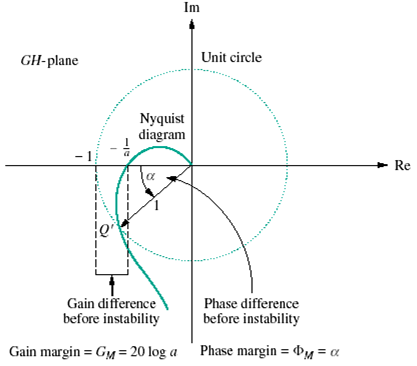
\includegraphics[width=\textwidth]{../pics/phase-margin.png}
			}
		\end{columns}
	\end{frame}

\section{Event-driven Sampling}
	\begin{frame}{Lebesgue vs Riemann}
		\begin{block}{Event-driven sampling}
			Also called ``Lebesgue sampling''
		\end{block}
		\vfill
		\begin{columns}
			\column{0.5\textwidth}
			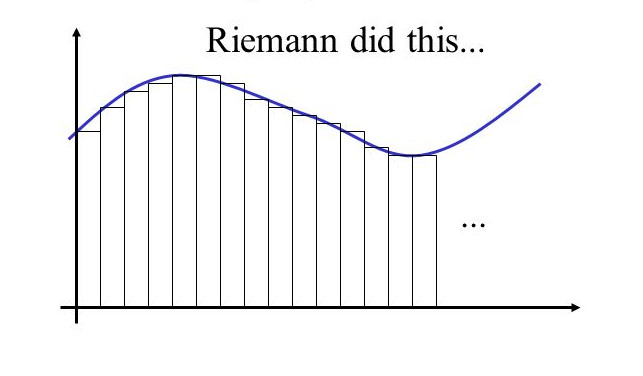
\includegraphics[width=\textwidth]{../pics/riemann_int_crop.jpg}
			\pause
			\column{0.5\textwidth}
			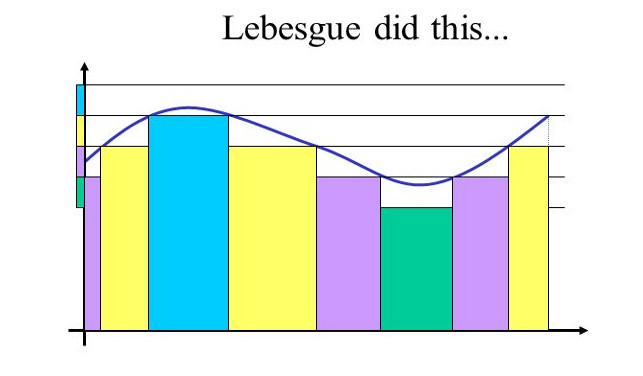
\includegraphics[width=\textwidth]{../pics/lebesgue_int_crop.jpg}
		\end{columns}
	\end{frame}

	\begin{frame}{Lebesgue sampling $\rightarrow$ Events}
		\only<1,2>{
			\centering
			\begin{tabular}{c}
				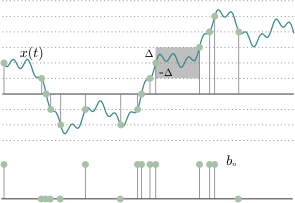
\includegraphics[width=0.6\textwidth]{../pics/lebesgue.png} \\
				\\
				\pause
				
\includegraphics[width=0.9\textwidth]{../pics/periodic_to_event_driven_4.png}
			\end{tabular}
		}

		\only<3>{
			\begin{description}[Sensor output]
			  \item[Event] Typically boolean ``message'' - a spike, or $\delta(t)$
				\item[Sensor output] \alert{Asynchronous} stream of events - a train of $\delta(t)$
			\end{description}
		}
	\end{frame}

	\begin{frame}{Some event-driven systems}
		\begin{columns}
			\column{0.7\textwidth}
			\begin{itemize}
				\item Position encoders
					\begin{itemize}
						\item Pulse when position has changed by specific amount
						\item[$\rightarrow$] \em{\small{Time encoding}}
					\end{itemize}
				\pause
				\item Pulse-frequency modulation
					\begin{itemize}
						\item Light-load DC-DC conversion
						\item[$\rightarrow$] \em{\small{Rate encoding}}
					\end{itemize}
				\pause
				\item Biological sensory organs
					\begin{itemize}
						\item Retina
						\item Cochlea
						\item[$\rightarrow$] \em{\small{Encoding?}} \small{Likely time and place}
					\end{itemize}
			\end{itemize}
			\column{0.3\textwidth}
			\includegraphics<3->[width=\textwidth]{../pics/retina.png} \\
			\includegraphics<3->[width=\textwidth]{../pics/cochlea.png}
		\end{columns}
		\pause
		\vskip15pt
		\begin{center}
			\fbox{\alert{Biological neurons!}}
		\end{center}
	\end{frame}

	\begin{frame}{Comparison of periodic \& event-driven control}
		\only<2,3>{$$ dx = u\thinspace dt + dv $$}
		\only<1>{
			\begin{block}{Definitions}
				The control attempts to keep the system state at the origin.
				Let the system to control be defined by:
				$$ dx = u\thinspace dt + dv $$
				where
				\begin{description}[$x$:]
					\item[$x$:] System state
					\item[$u$:] Control signal
					\item[$v$:] Disturbance (Wiener process)
					\item[$d$:] Lebesgue sampling interval
				\end{description}
			\end{block}
		}
		\only<2>{
			\begin{block}{Periodic sampling with period $h$}
			  Using a minimum variance controller, the control law becomes:
				$$ u = -\frac{1}{h} \frac{3 + \sqrt{3}}{2 + \sqrt{3}}\thinspace x $$
				and the variance becomes:
				$$ V_R = \frac{3 + \sqrt{3}}{6}\thinspace h $$
			\end{block}
		}
		\only<3>{
			\begin{block}{Event-driven sampling with mean period $h_L$}
			  Need different control strategy: an impulse that instantly returns the system to the origin.
				$T_d$ is the time it takes for $ |x(t_k)| = d $ for the 1st time.
				Mean exit time and mean sampling period:
				$$ h_L := E[T_d] = d^2 $$
				And the steady state variance:
				$$ V_L = \frac{d^2}{6} = \frac{h_L}{6} $$
			\end{block}
		}
		\only<4->{
			\begin{block}{Comparison}
			  To compare, assume the mean sampling rates are equal: $ h = h_L $. Then:
				$$ \frac{V_R}{V_L} = 4.7 $$
				But each follows a different control strategy to allow simple analysis. \\
				\visible<5->{
					Periodic sampling with impulse control as well:
					$$ \frac{V'_R}{V_L} = 3 $$
				}
			\end{block}
			\visible<5->{
				\centering
				\fbox{Event-driven sampling offers \em{3 times less variance}}

				The difference is even larger for unstable systems
			}
		}
	\end{frame}

	\begin{frame}{Consequences for control}
		Event signals are incompatible with traditional signal processing of continuous signals. But offer other benefits:
		\begin{itemize}
		  \item Take control action only as necessary - not on steady state!
			\item Same control efficiency with lower sampling rate
		\end{itemize}
	\end{frame}

\section{Dynamic Vision Sensor}

	\begin{frame}{From frames to events}
		\begin{block}{Normal camera}
			\pause
			\begin{itemize}
			  \item Rolling or global shutter
				\item Fixed frame rate
				\item Single pictures at constant rate
			\end{itemize}
		\end{block}
		\pause
		\begin{block}{Event-driven camera}
			\pause
			\begin{itemize}
				\item Independent pixels
				\item Each detects brightness change in its receptive field
				\begin{itemize}
					\item[--] \hskip5pt \spot<5->(1){\em{Logarithmic}} changes
					\item[]
					\item<5>[] \spot<5>(2){Fechner's Law}
						\tikz[remember picture,overlay]{ \draw (2) to[=>] (1); }
				\end{itemize}
				\pause
			\end{itemize}
		\end{block}
	\end{frame}

	\begin{frame}{From frames to events}
		\begin{block}{Event-driven camera}
			\begin{itemize}
				\item Independent pixels
				\item Each detects brightness change in its receptive field
				\begin{itemize}
					\item[--] \em{Logarithmic} changes
				\end{itemize}
				\item change $>$ threshold $\rightarrow$ event (asynchronous)
				\begin{itemize}
					\item[--] event: $e_k = {x_k,y_k,t_k,p_k}$ -- coordinates, timestamp \& polarity
				\end{itemize}
				\pause
				\item High temporal resolution (microseconds)
				\item Low spatial resolution ($~128\times 128 px$)
				\item Dynamic range $120dB$ vs. $~60dB$ for traditional image sensors
				\item Shared event bus
				\begin{itemize}
					\item[--] Statistical time division multiplexing
				\end{itemize}
			\end{itemize}

			\pause
			\centering
			\fbox{Asynchronous event stream instead of frames}
		\end{block}

	\end{frame}

	\begin{frame}{Event Processing}
		\begin{block}{Problem satisfaction}
			An event-driven sensor can address the issues stated at the beginning
			\begin{itemize}
				\item Low latency
				\item Little data redundancy
			\end{itemize}
		\end{block}

		\pause
		\begin{block}{Communication protocol}
		  Address Event Representation
		\end{block}

		\vskip10pt
		\framebox{\minibox{Requires different processing methods from standard sensors, \\
			based on spatio-temporal correlation}}
	\end{frame}

	\begin{frame}{Pseudo-simultaneity}
		\begin{columns}
			\column{0.5\textwidth}
			\begin{block}{Pseudo-simultaneity of event processing}
				Each event adds only little information, but is processed very fast,
				and the response time is not throttled by the frame rate.
				The output event stream lags behind the input only by a few events.
			\end{block}

			\column{0.5\textwidth}
			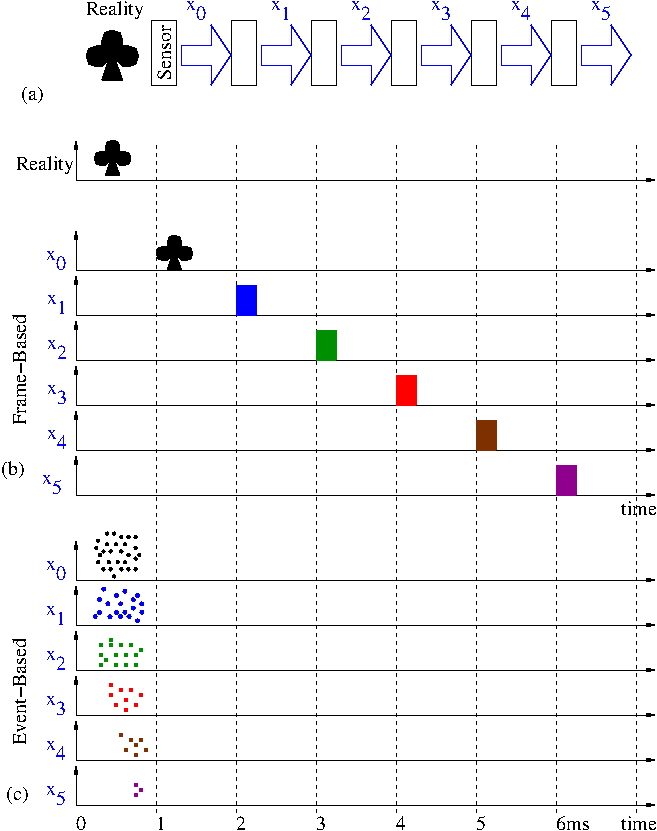
\includegraphics[width=0.9\textwidth]{../pics/pseudo-simultaneous_processing.png}
		\end{columns}
	\end{frame}

	\begin{frame}[c]{Example Visual Event Processor: Convolutional NN}
		\begin{columns}
			\column{0.7\textwidth}
			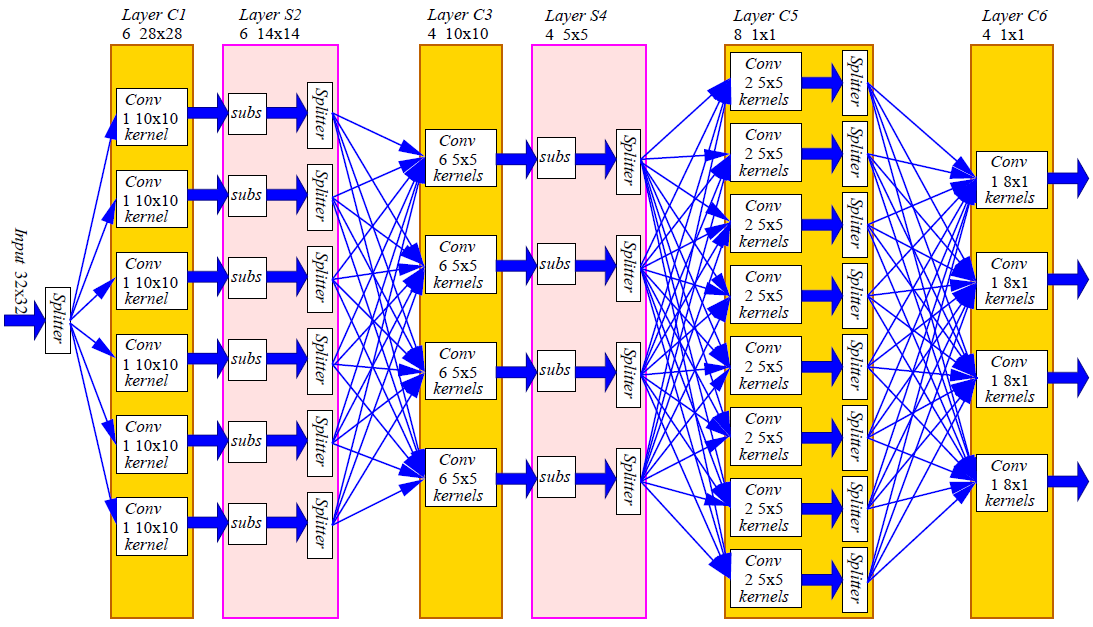
\includegraphics[width=\textwidth]{../pics/convnet.png}
			\column{0.3\textwidth}
			Implementations:
			\begin{enumerate}[<+->]
			  \item GPU
				\item FPGA
				\item Custom digital hardware
				\item Custom analog hardware
			\end{enumerate}
		\end{columns}
	\end{frame}

\section{Back to the Pencil Balancer}
	\begin{frame}{Pencil balancer description}
		\begin{block}{Visual balancing robots}
			\begin{description}[This one]
			  \item[Typical]
					\begin{itemize}
						\item[-] Frame-based sensors
						\item[-] Complex nonlinear control
					\end{itemize}
				\pause
				\item[This one]
					\begin{itemize}
						\item[-] Event-driven sensors
						\item[-] \alert{Simple PD control} (thanks to \em{low latency})
					\end{itemize}
			\end{description}
		\end{block}
		\vskip20pt

		\pause
		System elements:
		\begin{enumerate}
			\item Monitors object with 2 DVS
			\item Actuates with 2 independent servos
			\item Controls with linear PD algorithm
		\end{enumerate}
	\end{frame}

	\begin{frame}{Wrapping up with pencil balancer}
		\only<1>{
			\begin{center}
				\begin{tikzpicture}[->,>=stealth',shorten >=1pt,auto,node distance=4.5cm,
					thick,main node/.style={draw,font=\sffamily}]
					\node[main node] (1) {DVS};
					\node[main node] (2) [right of=1] {DVS ctl};
					\node[main node] (3) [below right of=2] {servo ctl};
					\node[main node] (4) [below left of=3] {servo ctl};
					\node[main node] (5) [left of=4]  {servo};
					\node[main node] (6) [below right of=1] {\textbf{Information Flow}};

					\path[every node/.style={font=\sffamily\small}]
					(1) edge node {events @$200kHz$} (2)
					(2) edge node {$(X,a)$ 2D line estimate @$2.5kHz$} (3)
					(3) edge node {$(X,Y,a_x,a_y)$ 3D line estimate} (4)
					(4) edge node {PD control @$500Hz$} (5);
				\end{tikzpicture}
			\end{center}
		}
		\only<2>{
			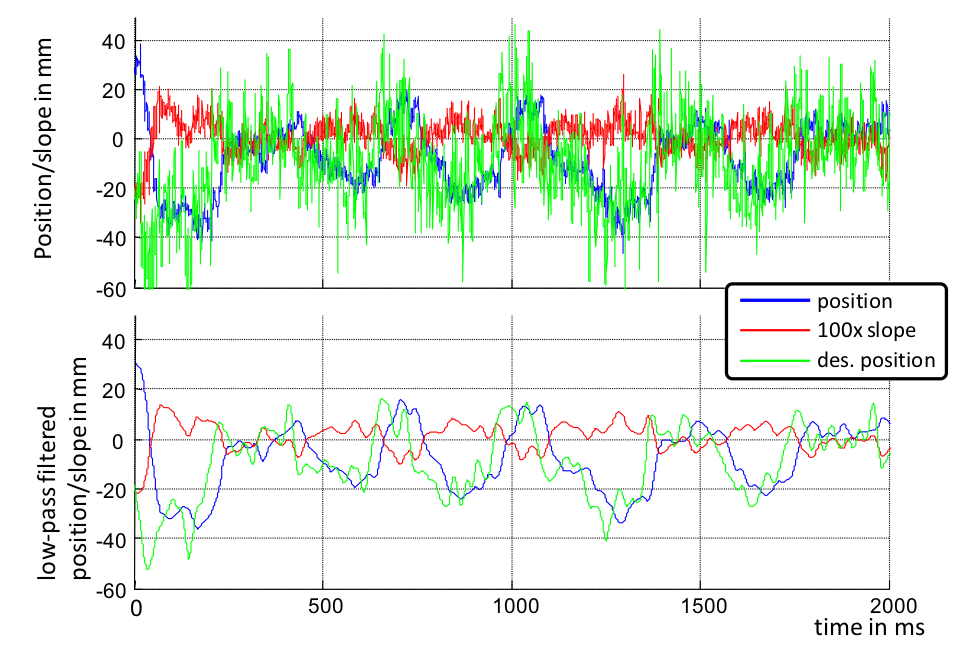
\includegraphics[width=0.8\textwidth]{../pics/pencil-control-res.png}
		}
	\end{frame}

	\begin{frame}[plain,c]
		\begin{center}
			\Large{\textbf{Thank you!}}
		\end{center}
	\end{frame}
	\begin{frame}[allowframebreaks]
		\frametitle{References}
		\begin{enumerate}
			\item Jonathan Tapson, Greg Cohen, Andre van Schaik, ``ELM solutions for event-based systems'',
				Neurocomputing, 13 Jan 2014
			\item K.J. Astrom, B.M. Bernhardsson, ``Comparison of Riemann and Lebesgue sampling for
				first order stochastic systems``, Proc. 41st IEEE Conf. Decis. Control 2
			\item Jorg Conradt, Raphael Berner, Matthew Cook, ``An Embedded AER Dynamic Vision Sensor for
				Low-Latency Pole Balancing'', IEEE 12th International Conference on Computer Vision
				Workshops, ICCV Workshops, 2009
			\item L. A. Camunas-Mesa, T. Serrano-Gotarredona, and B. Linares-Barranco, ``Event-Driven Sensing and Processing for
				High-Speed Robotic Vision''
			\item Shih-Chii Liu and Tobi Delbruck, ``Neuromorphic sensory systems'', Current Opinion in Neurobiology, 2010
		\end{enumerate}

	\end{frame}


\end{document}
